\begin{figure}[h!]
	\centering{
		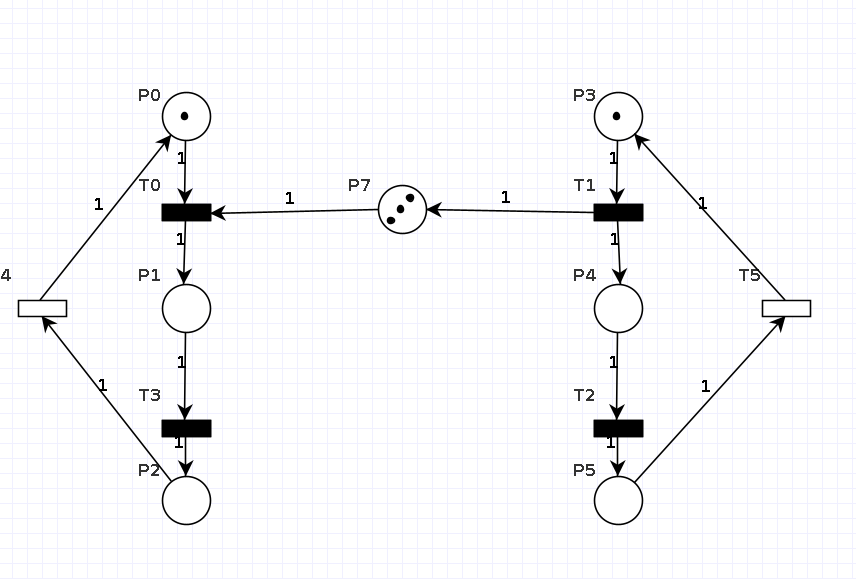
\includegraphics[width=0.67\textwidth]{img/buf2.png}
	}
	\caption{Sieć reprezentująca bufor nieograniczony}
	\label{zad2:graph1}
\end{figure}

\begin{figure}[h!]
	\centering{
		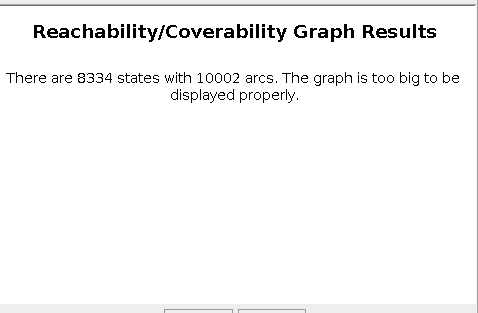
\includegraphics[width=0.67\textwidth]{img/buf2r.png}
	}
	\caption{Niezminniki sieci}
	\label{zad2:graph1}
\end{figure}

\subsection{Analiza niezmienników}
Można łatwo zaobserwować, że ze względu na bufor ($P_2$) sieć nie będzie ograniczona 
ani tym bardziej bezpieczna. 
Nie będzie także zachowawcza.

\subsection{Graf osiągalności}
Jak widzimy graf osiągalności jest za duży, żeby program go narysował. 
Czego warto było się spodziewać, gdyż sieć nie jest ograniczona.